\chapter{Etude technique}

\section*{Introduction}
La conception et la modélisation sont à la base du projet. Les connaître nous permettra de bien définir les autres composantes et besoins de ce projet. Cela comprend les choix techniques et les outils informatiques utilisés pour obtenir des résultats satisfaisants. C'est un projet  structuré avec des composants interconnectés pour un excellent flux de travail.

\section{Conception et modelisation}
Maintenant que nous avons décrit les phases du problème, concentrons-nous sur les phases fondamentales du cycle de vie du logiciel: les phases de conception et de modélisation. Le but de cette phase est de dériver une spécification pour l'architecture du système. 
Cette phase conduit à la conception et à la schématisation de classes et de séquences basées sur le langage de modélisation UML.

Dans tout ce qui précède, nous pouvons remarquer une structure légèrement différente de celle que nous avons déjà montrée dans la section \ref{Solution_prop}.
    \subsection{Structure générale du projet}
    Pour construire une nouvelle structure, il faut s'appuyer sur les points issus du chapitre précédent.

    Pour ce faire, on doit utiliser une base de données secondaire. Il s'agit d'une grande base de données structurée de la population adulte, pour construire des modéles pré-entraînés sur des donnéees de la population adulte, Un phénomène décidément très proche du nôtre.
    Après tous ces considérations on a trouver la structure du figure \ref{fig:structure_gen}
    \begin{figure}[H]
        \centering
        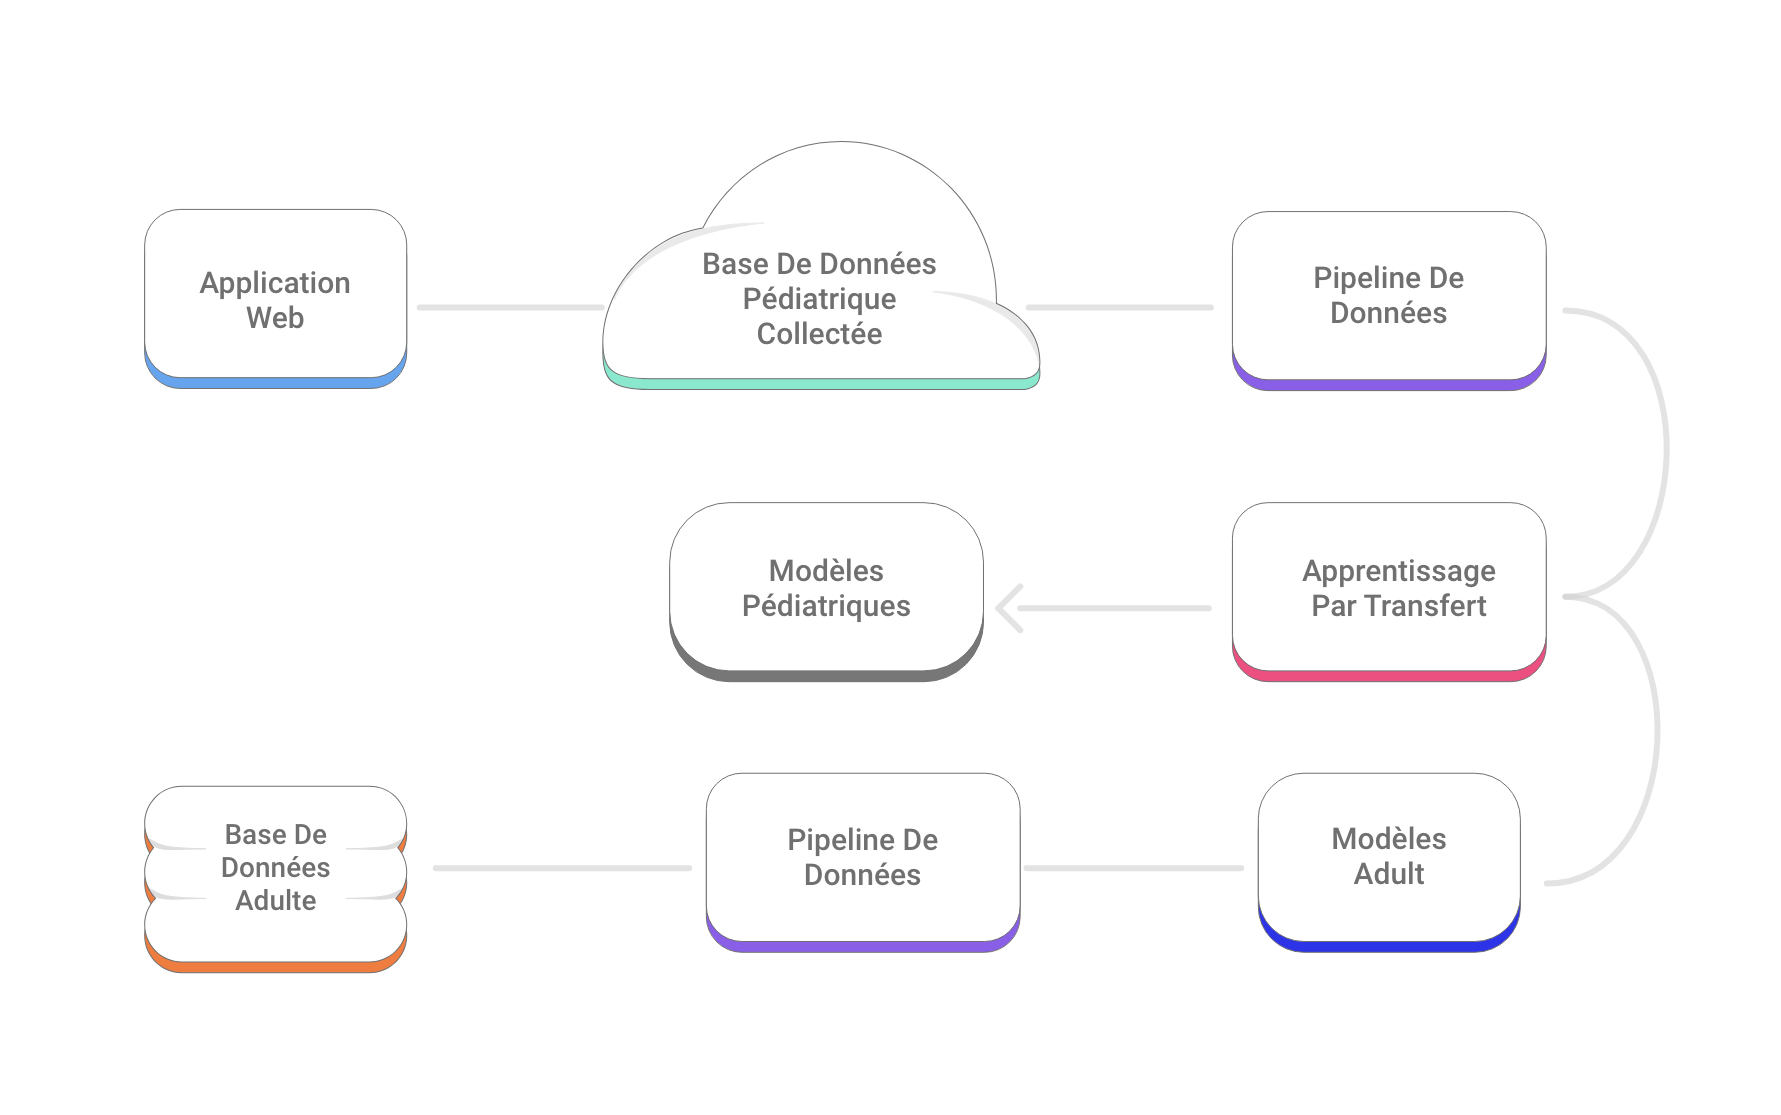
\includegraphics[width=0.7\textwidth]{structure_gen.jpg}
        \caption{structure génerale du projet}\label{fig:structure_gen}
    \end{figure}
    \subsection{Application Web}
        L'application Web est une API simple pour la collection et la visualisation de données, donc son architecture de base est également simple, c'est comme suit figure \ref{fig:xpedia_arc}
        \begin{figure}[H]
            \centering
            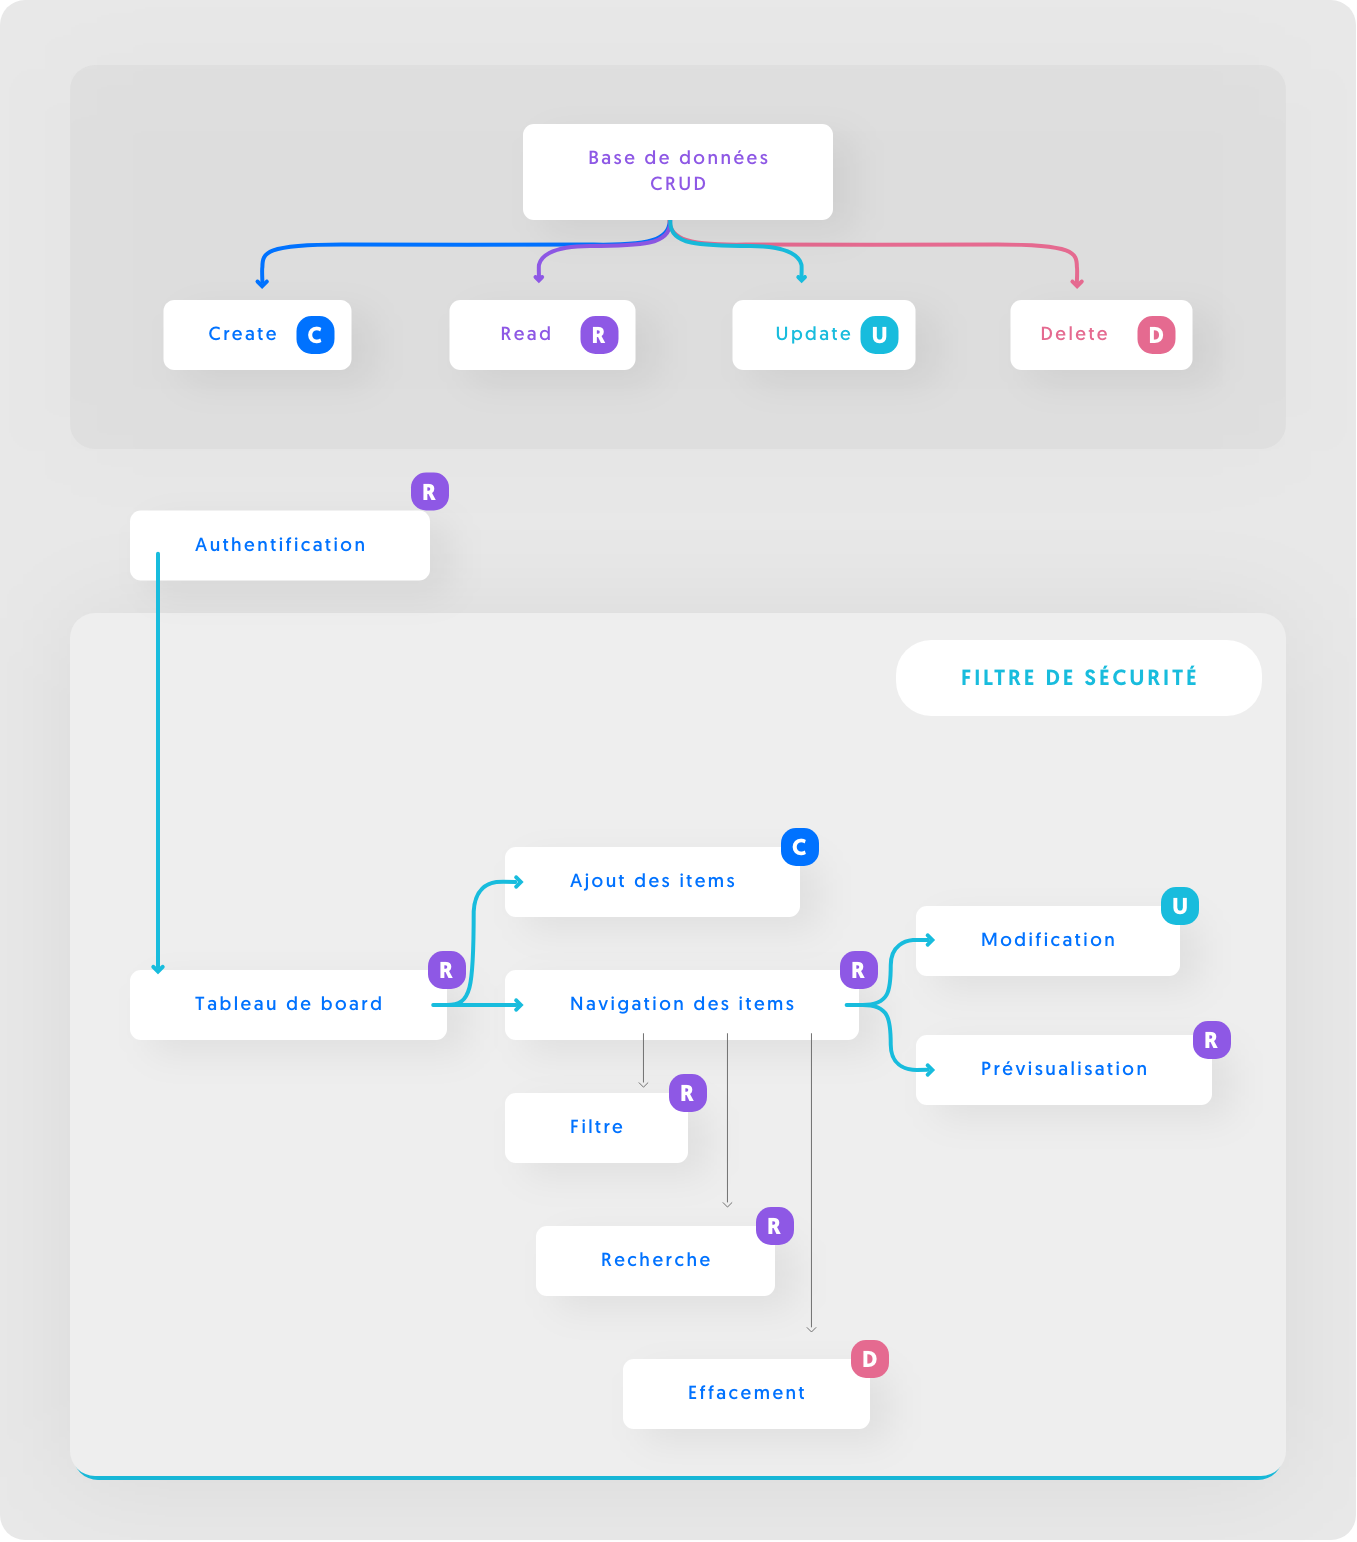
\includegraphics[width=1\textwidth]{xpedia_arc.png}
            \caption{structure génerale de l'application web Xpedia}\label{fig:xpedia_arc}
        \end{figure}
        \subsubsection{UML}
            UML (abréviation de Unified Modeling Language) est un langage de modélisation standardisé composé d'un ensemble de diagrammes intégrés qui aident les développeurs de systèmes et de logiciels à spécifier, visualiser et visualiser les artefacts des systèmes logiciels. .système. UML représente un ensemble éprouvé de meilleures pratiques techniques pour la modélisation de systèmes vastes et complexes et constitue une partie très importante du développement logiciel orienté objet et du processus de développement logiciel. UML utilise principalement une notation graphique pour représenter la conception de projets logiciels.

            \begin{enumerate}
                \item Diagramme de classe:
                Notre diagramme de classe de  deux classes utilisateur et xray (cliché), notre but de cette application et de collectés les données (xrays), l'acteur qui va effectuer la collection est l'utilisateur:
                \begin{figure}[H]
                    \centering
                    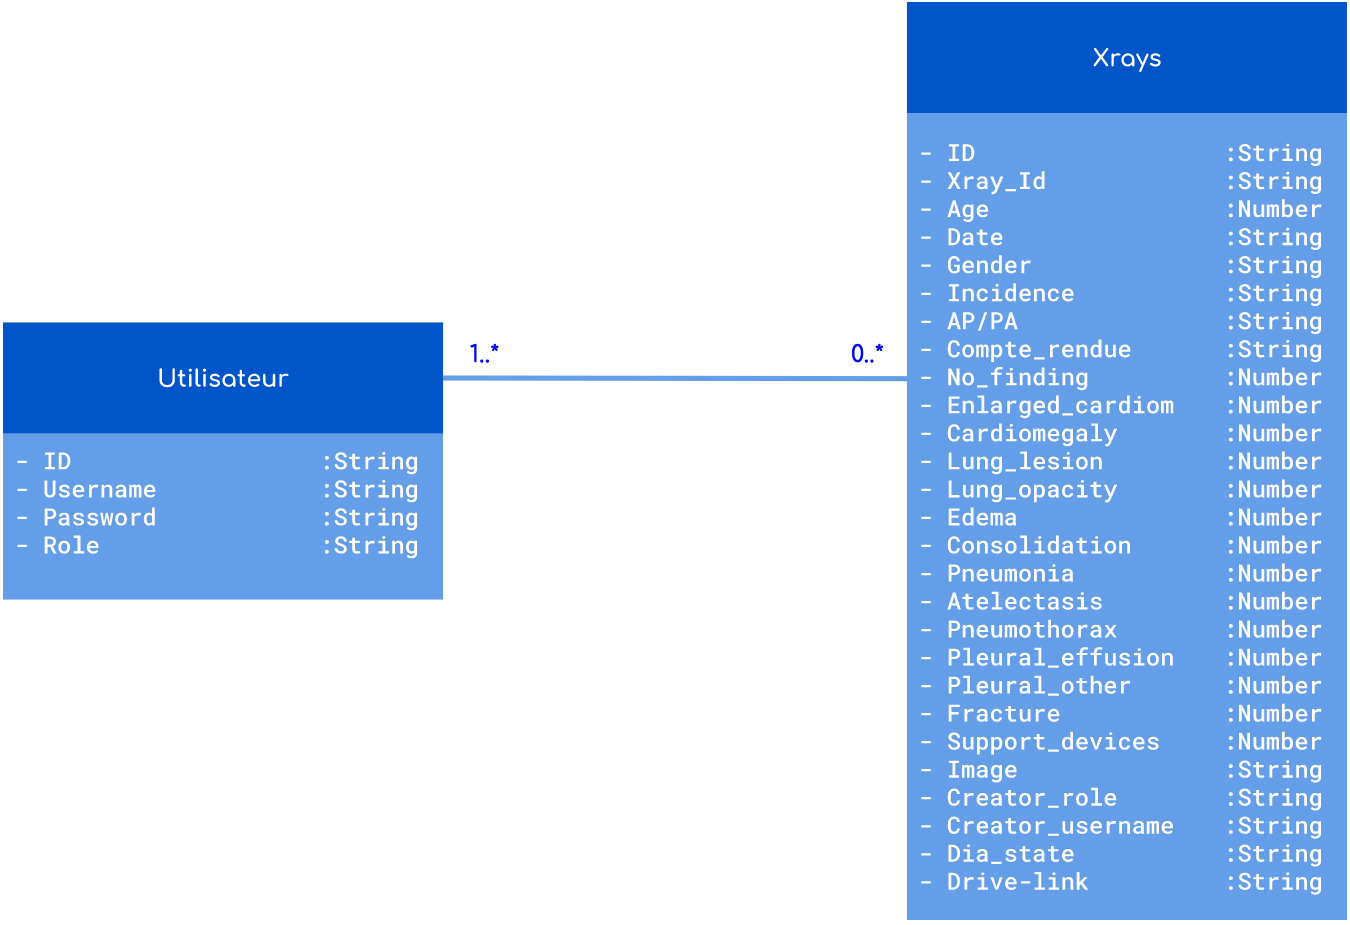
\includegraphics[width=0.8\textwidth]{class_dia.png}
                    \caption{Le diagramme de classe de l'application web Xpedia}\label{fig:class_dia}
                \end{figure}

                \item Diagrammes de séquence
                
                Un diagramme de séquence représente les objets impliqués dans une interaction particulière et les messages qu'ils échangent organisés par ordre chronologique.
                \begin{enumerate}
                    \item Diagramme de séquence: cas d'authentification
                    \begin{figure}[H]
                        \centering
                        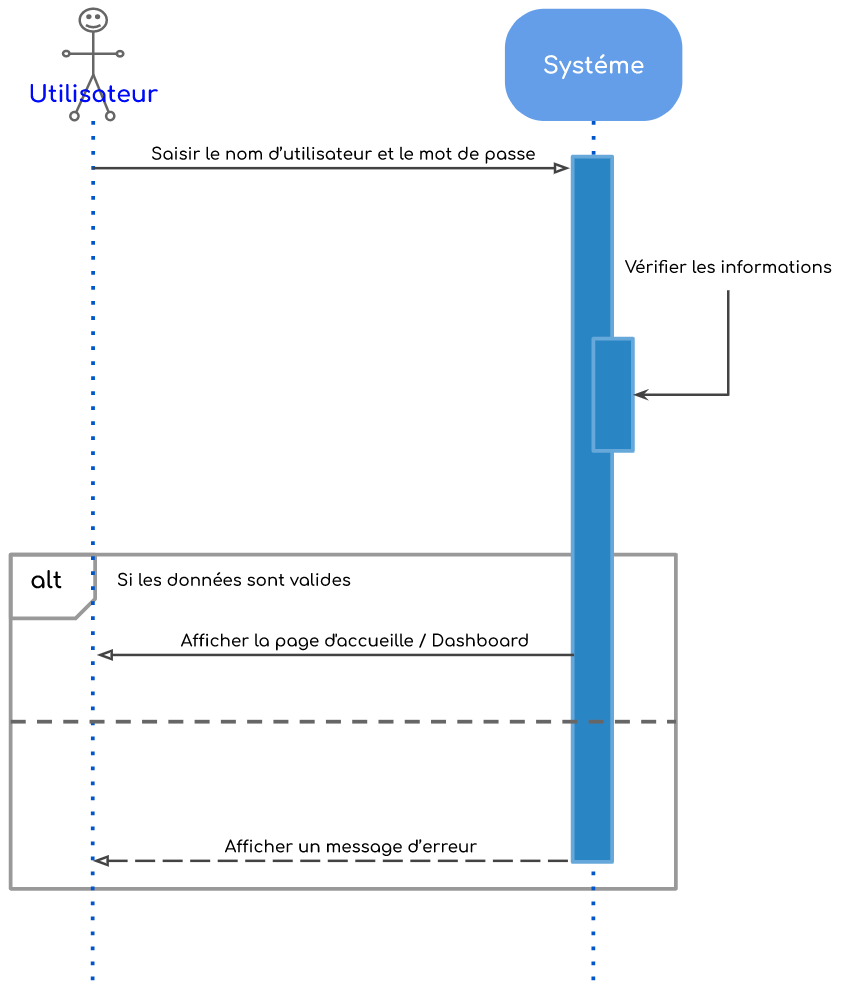
\includegraphics[width=0.5\textwidth]{cas_auth.png}
                        \caption{Le diagramme de séquence: cas d'authentification}\label{fig:cas_auth}
                    \end{figure}

                    Comme on peut le voir sur la figure \ref{fig:cas_auth}, l'authentification se fait à travers 2 opérations principales:
                    \begin{itemize}[label=$\bullet$]
                        \item l'utilisateur fournit le nom d'utilisateur et le mot de passe
                        \item le système recoupe les informations fournies avec les données existantes dans la collection de l'utilisateur
                    \end{itemize}
                    \item Diagramme de séquence: cas d'ajouter un cliché
                    \begin{figure}[H]
                        \centering
                        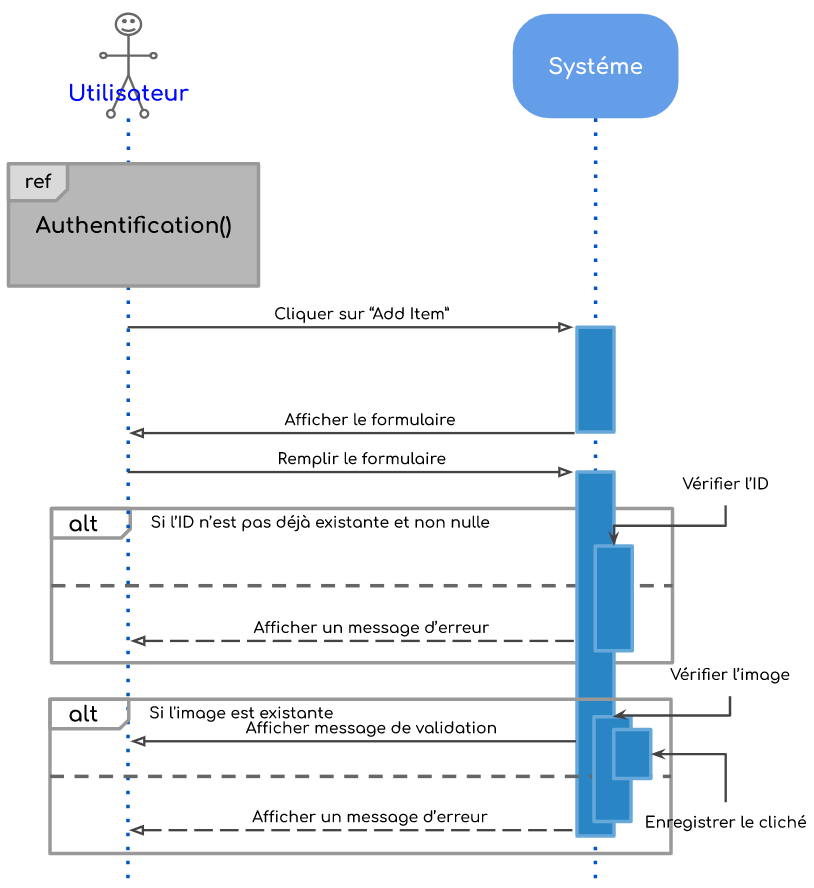
\includegraphics[width=0.5\textwidth]{cas_add.png}
                        \caption{Le diagramme de séquence: cas d'ajouter un cliché}\label{fig:cas_add}
                    \end{figure}
                \end{enumerate}
            \end{enumerate}
        
    \subsection{Pipeline de données}
    \paragraph*{Un pipeline de données est} une série d'étapes de traitement de données. Si les données ne sont pas actuellement chargées dans la plateforme de données, elles seront ingérées au début du pipeline. Ensuite, vous avez une séquence d'étapes où chaque étape fournit une sortie qui devient l'entrée de l'étape suivante. Cela continue jusqu'à ce que le pipeline soit terminé. Dans certains cas, des étapes indépendantes peuvent s'exécuter en parallèle.  
    
    Un pipeline de donnéesse compose de trois éléments principaux : une source, une ou plusieurs étapes de traitement et une destination. Dans certains pipelines de données, une destination peut être appelée un récepteur. Par exemple, un pipeline de données peut transmettre des données de votre application à un entrepôt de données, d'un lac de données à une base de données d'analyse ou à un système de traitement des paiements. Un pipeline de données peut également avoir la même source et le même récepteur, de sorte que le pipeline n'a besoin que de modifier l'ensemble de données. Chaque fois que des données sont traitées entre le point A et le point B (ou les points B, C, D), il existe un pipeline de données entre ces points.

        \subsubsection{Integration}
        L'intégration de données est le processus consistant à combiner des données provenant de différentes sources en une vue unique et unifiée. L'intégration commence par le processus d'ingestion et comprend des étapes telles que le nettoyage, le mappage ETL et la transformation. L'intégration des données permet finalement aux outils d'analyse de produire une intelligence économique efficace et exploitable.

        Il n'existe pas d'approche universelle de l'intégration des données. Cependant, les solutions d'intégration de données impliquent généralement quelques éléments communs, notamment un réseau de sources de données, un serveur maître et des clients accédant aux données à partir du serveur maître.

        Dans un processus d'intégration de données typique, le client envoie une demande de données au serveur maître. Le serveur maître reçoit ensuite les données nécessaires à partir de sources internes et externes. Les données sont extraites des sources, puis consolidées en un seul ensemble de données cohérent. Ceci est renvoyé au client pour utilisation.
        \subsubsection{Transformation}
        La transformation des données est le processus de transformation des données d'un format à un autre. Généralement, vous convertissez du format du système source au format requis par le système cible. Les transformations de  données font partie de la plupart des tâches d'intégration et de gestion des données, telles que : B. Gestion des données et stockage des données. 

        En tant qu'étape du processus ELT/ETL, la transformation des données peut être qualifiée de « simple » ou de « complexe » selon le type de modifications qui doivent être apportées aux données avant qu'elles ne soient livrées à leur destination. Le processus de transformation des données peut être effectué à l'aide de l'automatisation, de l'administration manuelle ou d'une combinaison des deux.

        \subsubsection{Réduction}
        La réduction des données signifie la réduction de certains aspects des données, généralement le volume de données. La réduction peut également porter sur d'autres aspects tels que la dimensionnalité des données lorsque les données sont multidimensionnelles. La réduction de tout aspect des données implique généralement une réduction du volume de données.

        La réduction des données n'a de sens en soi que si elle est associée à une certaine finalité. Le but à son tour dicte les exigences pour les techniques de réduction de données correspondantes. Un but naïf de la réduction des données est de réduire l'espace de stockage. Cela nécessite une technique pour compresser les données dans un format plus compact et également pour restaurer les données d'origine lorsque les données doivent être examinées. De nos jours, l'espace de stockage n'est peut-être pas la principale préoccupation et les besoins de réduction des données proviennent fréquemment des applications de base de données. Dans ce cas, le but de la réduction des données est d'économiser le coût de calcul ou le coût d'accès au disque dans le traitement des requêtes.
        \subsubsection{Nettoyage}
        Le nettoyage des données est le processus de réparation ou de suppression des données incorrectes, corrompues, mal formées, en double ou incomplètes dans un ensemble de données. La combinaison de plusieurs sources de données augmente le risque de dupliquer ou de mal étiqueter les données. Si les données sont erronées, même si elles semblent correctes, les résultats et les algorithmes ne seront pas fiables. Il n'existe aucun moyen absolu de dicter les étapes exactes du processus de nettoyage des données, car le processus est différent pour chaque ensemble de données. Cependant, il est important de définir un modèle pour votre processus de nettoyage des données et de vous assurer que vous le faites correctement à chaque fois.


   
    \subsection{Modèles de deeplearning}

    \begin{figure}[H]
        \centering
        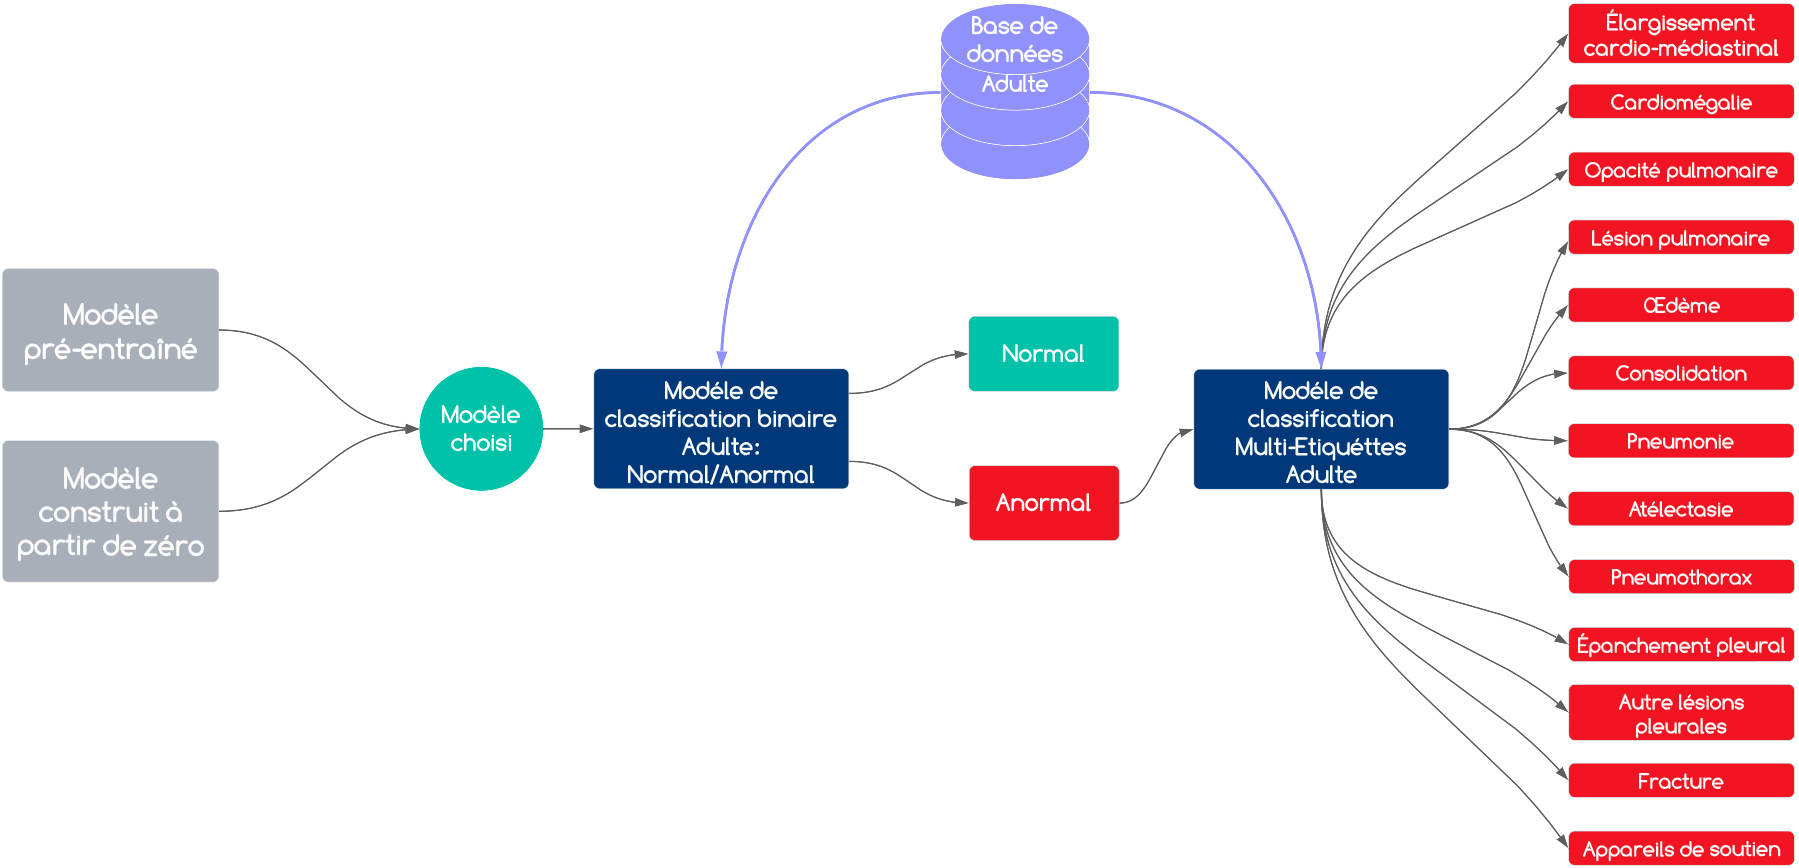
\includegraphics[width=1\textwidth]{adulte_model_train.png}
        \caption{La schéma de créeation du modèle des radiographies adultes}\label{fig:adulte_model_schema}
    \end{figure}
    \begin{figure}[H]
        \centering
        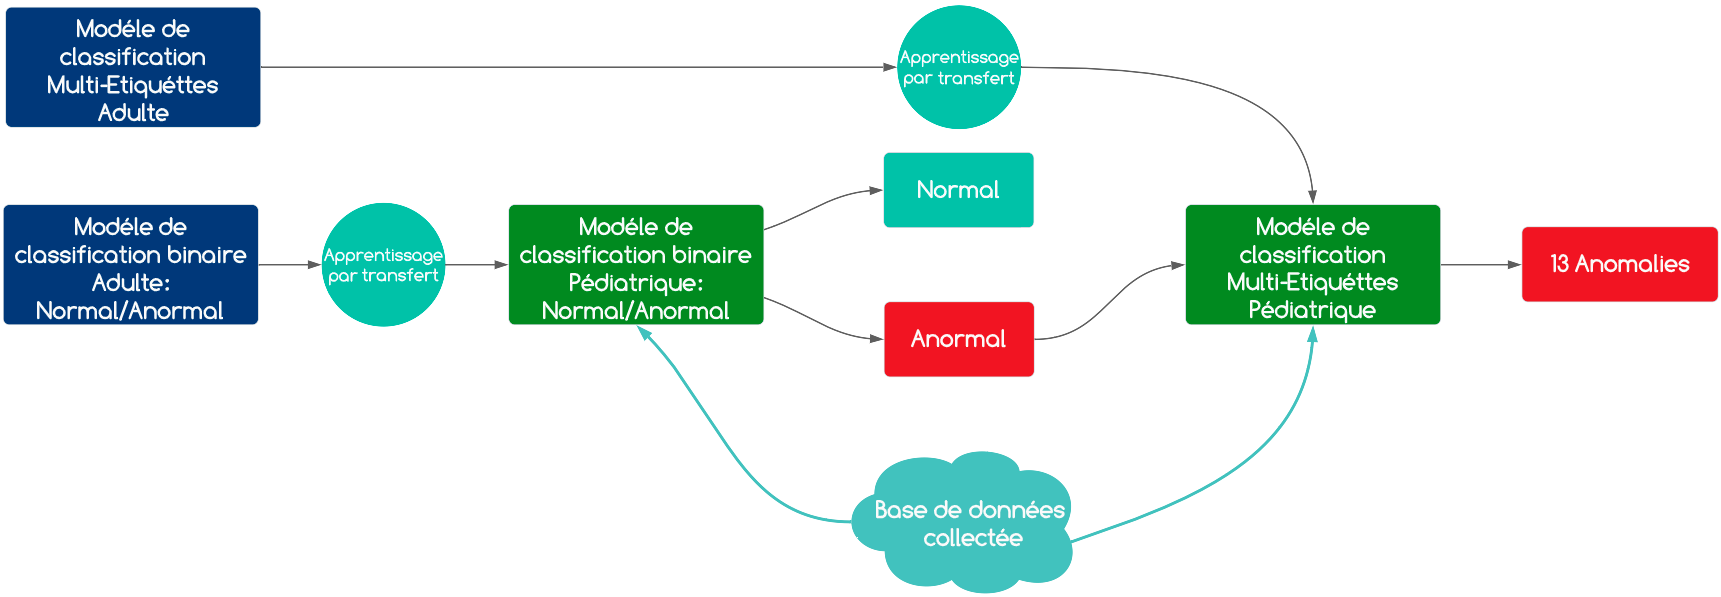
\includegraphics[width=1\textwidth]{pedia_model_train.png}
        \caption{La schéma de créeation du modèle des radiographies adultes}\label{fig:pedia_model_schema}
    \end{figure}
\section{Choix techniques}
Cette partie est consacrée à la présentation de l'environnement matériel et logiciel utilisé pour développer la solution proposée. Expliquer les décisions techniques concernant les langages de programmation et les outils à utiliser.
    \subsection{Architecture logicielle}
    \subsection{API}
    API signifie Application Programming Interface. En termes simples, une API est un ensemble de fonctions et de procédures qui vous permettent de créer une application. Accéder aux données et fonctionnalités d'autres applications, services ou systèmes d'exploitation. 
    Vous êtes essentiellement un intermédiaire entre différentes plates-formes logicielles. Ils permettent à deux applications indépendantes de "parler" entre elles. 
    Par exemple, supposons que vous êtes un agent de change fortement impliqué dans les marchés financiers et le trading. L'API peut lier un ensemble d'algorithmes de trading automatisés à la plateforme de courtage de trading préférée d'un trader. Il permet aux traders de visualiser les cotations et les données de prix en temps réel, ainsi que d'effectuer des transactions électroniques.

    \begin{figure}[H]
        \centering
        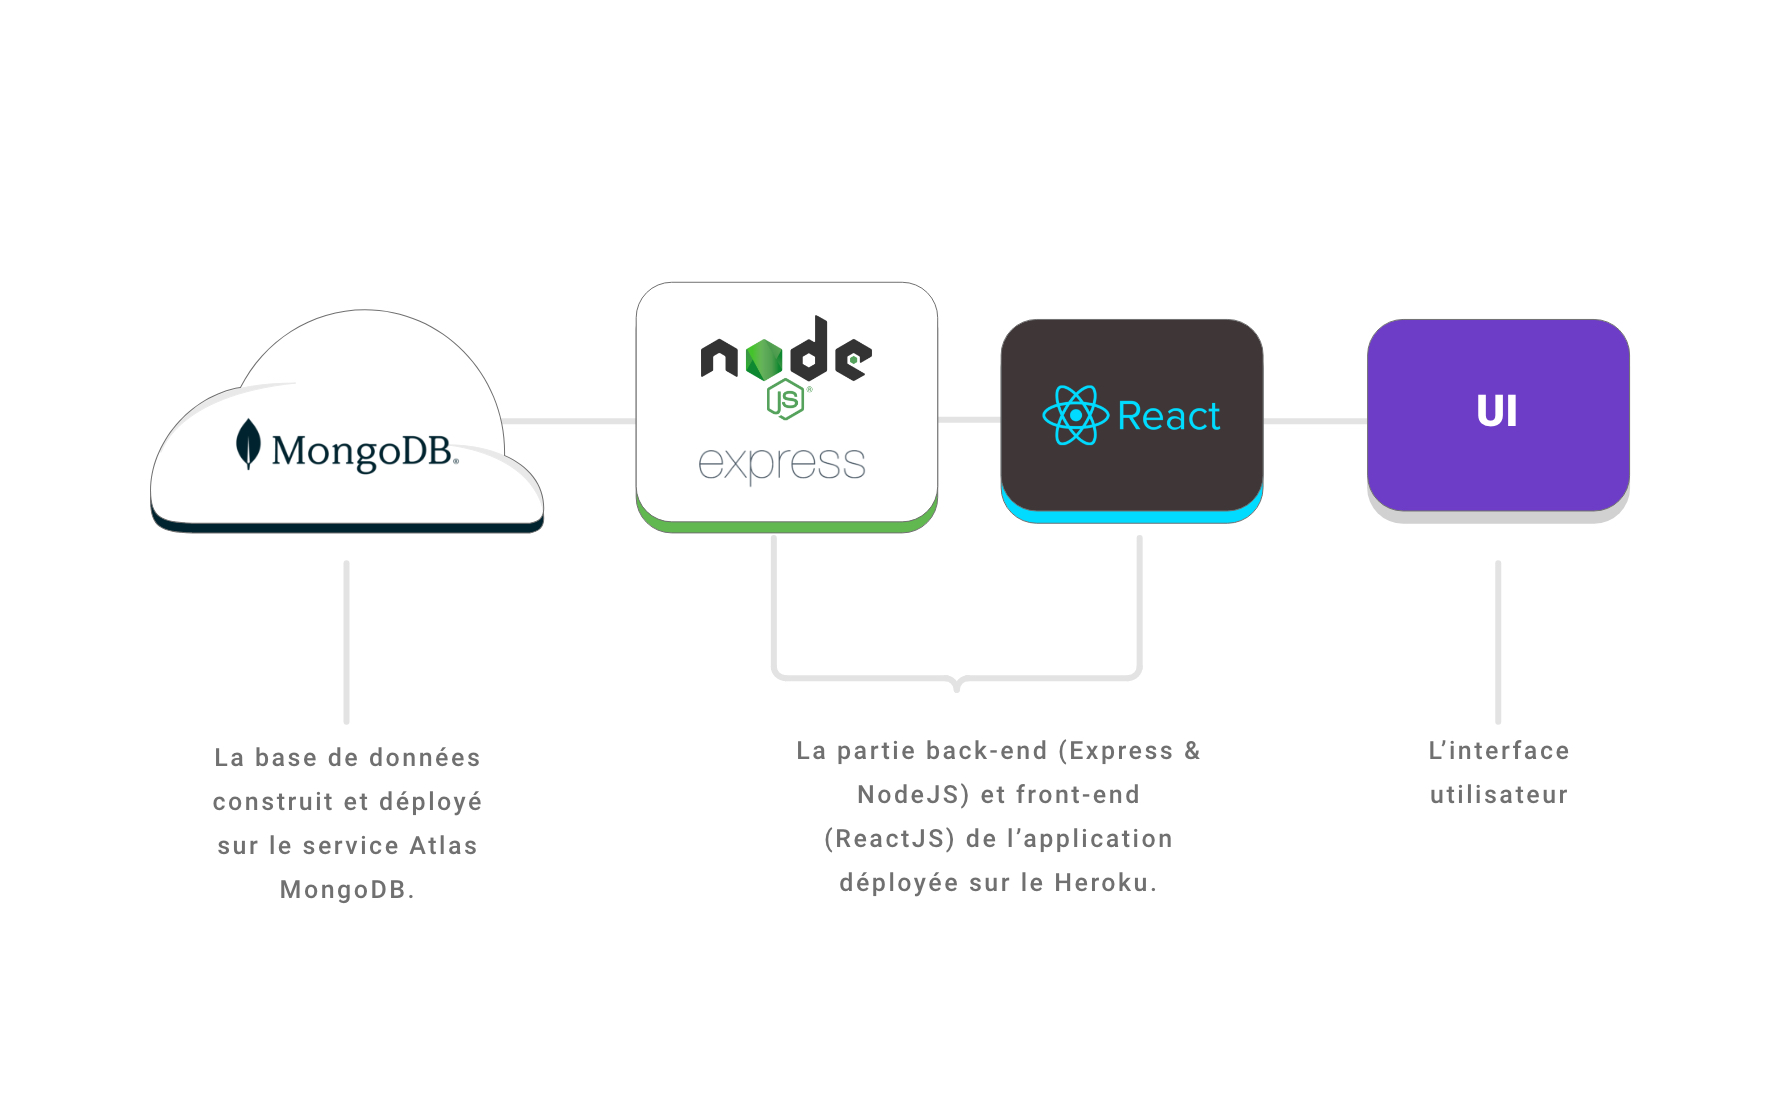
\includegraphics[width=1\textwidth]{log_arc.jpg}
        \caption{La schéma de logicielle de l'application web Xpedia}\label{fig:log_arc}
    \end{figure}

    \subsubsection{MERN stack}
    \begin{figure}[H]
        \centering
        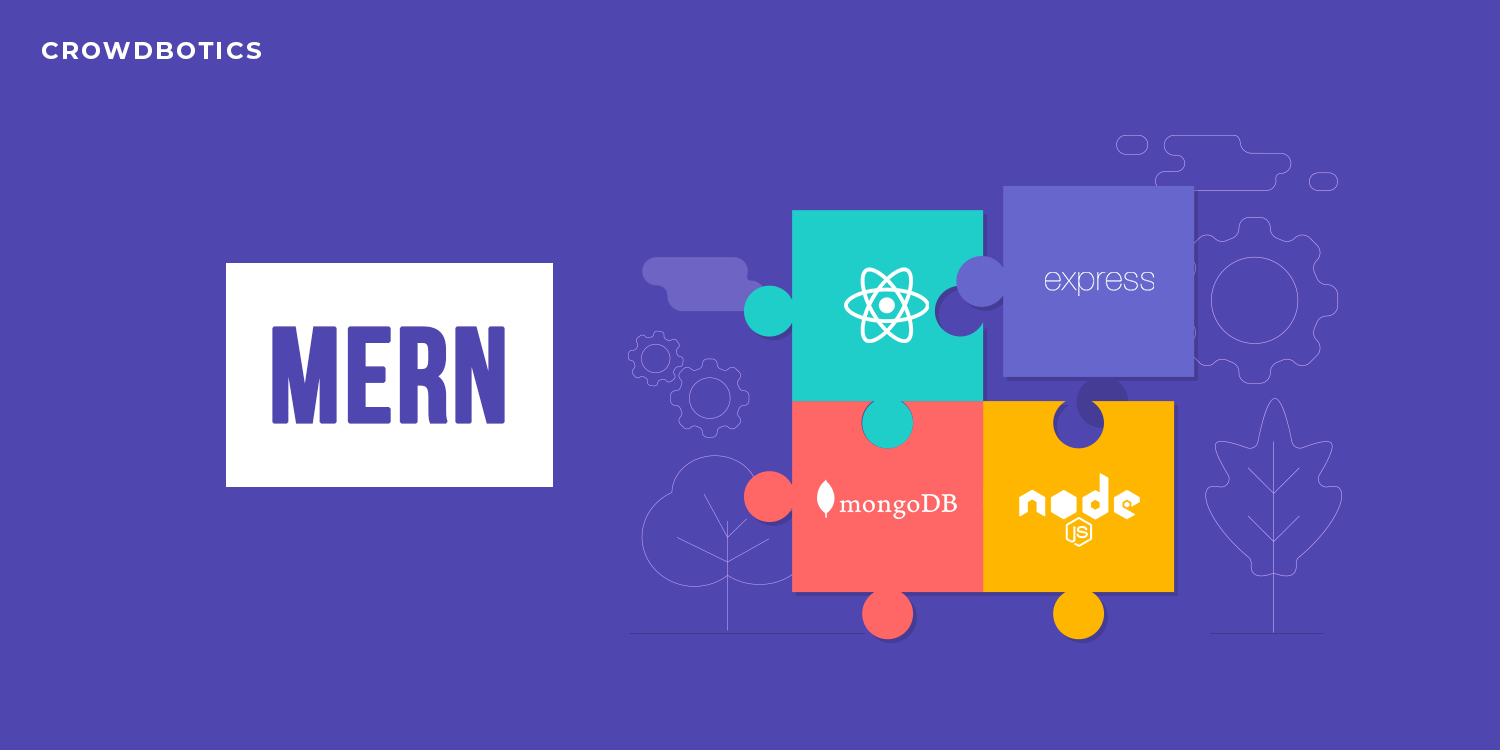
\includegraphics[width=0.6\textwidth, trim={5cm, 3cm, 5cm, 5cm},clip]{MERN.png}
        \caption{Le logo du MERN stack}\label{fig:mern}
    \end{figure}
    \paragraph{MERN Stack} est un ensemble de technologies puissantes et fiables utilisées pour développer des applications informatiques évolutives qui incluent des composants back-end, front-end et de base de données. JavaScript est utilisé pour développer des sites Web entiers plus rapidement et plus facilement.

    C'est une technologie qui est un framework JavaScript complet et convivial pour la création d'applications et de sites Web dynamiques.

    \paragraph{Pour quoi MERN?}MERN stack séparé en deux composants: le back-end et le front-end. De plus, l'ensemble du système de base de données est isolé du reste.

    L'ensemble du système, y compris le front-end, le back-end et la base de données, utilise l'API REST, qui agit comme un "middleware" et est réutilisable pour toute autre application: logiciel mobile, etc., très facilement.

    L'API REST vous permet de connecter des applications entre elles comme les pièces d'un puzzle. Les API REST sont basées sur HTTP et imitent les styles de communication Web, ce qui les rend très avantageuses à utiliser dans MERN.
    \begin{enumerate}\bfseries
        \item Atlas MongoDB\newline
        \begin{figure}[H]
            \centering
            
\includegraphics[width=0.6\textwidth]{atlass_mdb.png}
            \caption{Logo de Atlas MongoDB}\label{fig:atlass_mdb}
        \end{figure}
        \normalfont
        MongoDB Atlas est une plateforme de données de développeur multi-cloud. Au cœur se trouve notre base de données cloud entièrement gérée pour les applications modernes. Atlas est le meilleur moyen d'exécuter MongoDB, la principale base de données non relationnelle. Le modèle de document de MongoDB est le moyen le plus rapide d'innover car les documents correspondent directement aux objets de votre code. En conséquence, ils sont beaucoup plus faciles et plus naturels à travailler. Vous pouvez stocker des données de n'importe quelle structure et modifier votre schéma à tout moment lorsque vous ajoutez de nouvelles fonctionnalités à vos applications.

        Atlas Database est disponible dans plus de 80 régions sur AWS, Google Cloud et Azure. Vous pouvez même tirer parti des déploiements multi-cloud et multi-régions, ce qui vous permet de cibler les fournisseurs et les régions qui servent le mieux vos utilisateurs. Une automatisation de pointe et des pratiques éprouvées garantissent la disponibilité, l'évolutivité et la conformité aux normes de sécurité et de confidentialité des données les plus exigeantes.
        \bfseries
        \item Express Node js\newline
        \begin{figure}[H]
            \centering
            
\includegraphics[width=0.6\textwidth]{react.png}
            \caption{Logo de ReactJS}\label{fig:react}
        \end{figure}
        \normalfont
        Express est un cadre d'application Web Node.js minimal et flexible qui fournit un ensemble  de fonctionnalités robustes pour les applications Web et mobiles. 
        Express fournit une fine couche de fonctionnalités d'application Web de base sans masquer les fonctionnalités familières de Node.js.
        \bfseries
        \item React\newline
        \begin{figure}[H]
            \centering
            
\includegraphics[width=0.6\textwidth]{react.png}
            \caption{Logo de ReactJS}\label{fig:react}
        \end{figure}
        \normalfont
        React est une bibliothèque JavaScript pour créer des interfaces utilisateur. 

        Déclaratif: React facilite la création d'interfaces utilisateur interactives. Concevez une vue simple pour chaque état de votre application et React mettra à jour et affichera efficacement le composant approprié à mesure que les  données changent. Une vue déclarative rend votre code plus prévisible, plus facile à comprendre et plus facile à déboguer. 
 
        Basé sur les composants: créez des composants encapsulés qui gèrent leur propre état et combinez-les pour créer des interfaces utilisateur complexes. Étant donné que la logique des composants est écrite en JavaScript au lieu de modèles, vous pouvez facilement transmettre de grandes quantités de données  via votre application et conserver l'état en dehors du DOM.
 
        Apprenez une fois, écrivez n'importe où: nous ne faisons aucune hypothèse sur le reste de la pile technologique, vous pouvez donc développer de nouvelles fonctionnalités dans React sans réécrire le code existant. React peut également utiliser Node pour le rendu sur le serveur  et React Native pour exécuter des applications mobiles.

        \bfseries
    \end{enumerate}
    \subsubsection{Heroku}
    \begin{figure}[H]
        \centering
        
\includegraphics[width=0.6\textwidth]{heroku.png}
        \caption{Logo de Heroku}\label{fig:heroku}
    \end{figure}

    Heroku est une plate-forme de services cloud qui a gagné en popularité  ces dernières années. Heroku est si facile à utiliser qu'il est devenu le choix incontournable pour de nombreux projets de développement. 
    L'accent mis sur la prise en charge des applications centrées sur le client facilite le développement et le déploiement  des applications. Les entreprises utilisant Heroku peuvent se concentrer sur le perfectionnement de leurs applications, tandis que la plateforme Heroku gère le matériel et les serveurs. Ce n'est pas l'infrastructure qui les soutient.

    \subsubsection{VScode}
    \begin{figure}[H]
        \centering
        
\includegraphics[width=0.6\textwidth]{vscode.png}
        \caption{Logo de Visual Studio Code}\label{fig:vscode}
    \end{figure}

    \subsection{Architecture des réseaux de neurones}
    \subsubsection{Python}
    \begin{figure}[H]
        \centering
        
\includegraphics[width=0.6\textwidth]{python.png}
        \caption{Logo de Python}\label{fig:python}
    \end{figure}
    \subsubsection{Librairies}
    \begin{enumerate}\bfseries
        \item Numpy
        \begin{figure}[H]
            \centering
            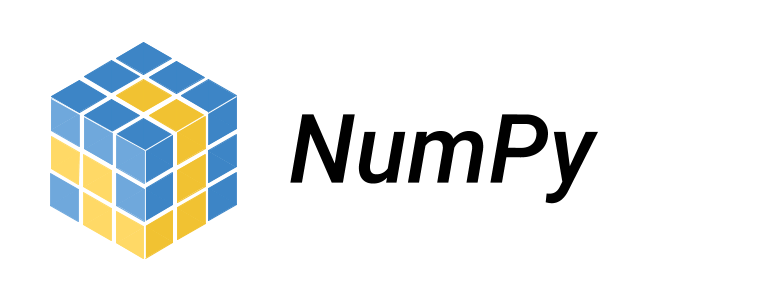
\includegraphics[width=0.6\textwidth]{numpy.png}
            \caption{Logo de Numpy}\label{fig:numpy}
        \end{figure}
        \normalfont

        \bfseries
        \item Pandas
        \begin{figure}[H]
            \centering
            
\includegraphics[width=0.6\textwidth]{pandas.png}
            \caption{Logo de Pandas}\label{fig:pandas}
        \end{figure}
        \normalfont

        \bfseries
        \item OpenCV
        \begin{figure}[H]
            \centering
            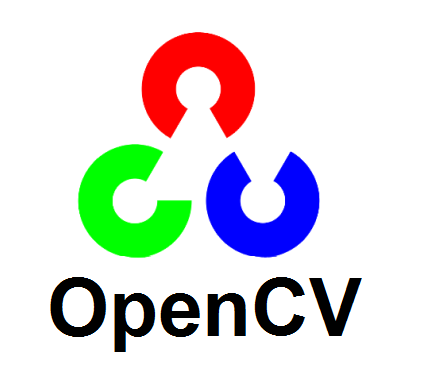
\includegraphics[width=0.6\textwidth]{opencv.png}
            \caption{Logo de Open Computer Vision}\label{fig:opencv}
        \end{figure}
        \normalfont

        \bfseries
        \item Tensorflow
        \begin{figure}[H]
            \centering
            
\includegraphics[width=0.6\textwidth]{tensorflow.png}
            \caption{Logo de Tensorflow}\label{fig:tensorflow}
        \end{figure}
        \normalfont

        \bfseries
        \item Keras
        \begin{figure}[H]
            \centering
            
\includegraphics[width=0.6\textwidth]{keras.png}
            \caption{Logo de Keras}\label{fig:keras}
        \end{figure}
        \normalfont

        \bfseries
        \item Matplotlib
        \begin{figure}[H]
            \centering
            
\includegraphics[width=0.6\textwidth]{matplotlib.jpeg}
            \caption{Logo de Matplotlib}\label{fig:matplotlib}
        \end{figure}
        \normalfont

        \bfseries
    \end{enumerate}
    \subsubsection{IDEs}
    \begin{enumerate}\bfseries
        \item Jupyter
        \begin{figure}[H]
            \centering
            
\includegraphics[width=0.6\textwidth]{jupyter.jpeg}
            \caption{Logo de Jupyter}\label{fig:jupyter}
        \end{figure}
        \normalfont

        \bfseries
        \item Google Colab pro+
        \begin{figure}[H]
            \centering
            
\includegraphics[width=0.6\textwidth]{colab.png}
            \caption{Logo de Colab}\label{fig:colab}
        \end{figure}
        \normalfont

        \bfseries
    \end{enumerate}
    \subsubsection{HPC-MARWAN}
    \begin{figure}[H]
        \centering
        
\includegraphics[width=0.6\textwidth]{marwan-hpc.png}
        \caption{Logo de HPC-MARWAN}\label{fig:marwan-hpc}
    \end{figure}

\section{Bases de données}
    \subsection{CheXpertDB}\label{chexpertDB}
    \subsection{XpediaDB}

\section*{Conclusion}